\section{Lesson 07 --- 22/10/2026}

\subsection{Rule-based Classification}
The idea is to use a set of rules to determine the class of an entity. We can use IF-THEN rules, for example
\begin{center}
  IF \s{age} = youth AND \s{student} = yes THEN \s{buys\_computer} = yes.
\end{center}
How can we measure if a rule is good? We can use \g{accuracy} to measure how many of the tuples that activate the rule are correctly classified. Another metric is the \g{coverage}: it measures how much of the dataset is covered by a rule. If a rule applies to only one tuple it is not a good rule (but it will have 100\% accuracy).

\begin{definition}[Coverage and accuracy]
Let $R$ be a rule, $D$ the dataset, $n_{covers}$ the number of tuples covered by $R$ and $n_{correct}$ the number of those tuples that $R$ classifies correctly. Then
\[
  coverage(R) = \frac{n_{covers}}{|D|}, \qquad accuracy(R) = \frac{n_{correct}}{n_{covers}}.
\]
\end{definition}

A problem with rule-based classification is that we could have a conflict if more than one rule fires for an instance. To deal with conflicts we can use priorities:
\begin{itemize}
  \item \g{Size ordering}: we give the highest priority to the rules with the toughest requirements, i.e.\ the most attribute tests in the antecedent.
  \item \g{Class-based ordering}: we order the classes by prevalence (rules for the most frequent class come first) or by misclassification cost (rules for the class with the highest cost come first).
  \item \g{Rule-based ordering}: we put the rules in a list ordered by rule quality (accuracy, coverage, size or domain advice) and apply them in order, like an access control list. This list is called a \s{decision list}.
\end{itemize}

\subsubsection{Rules from decision trees}
We can easily extract rules from a decision tree: each path from the root to a leaf becomes one rule.

\begin{example}
Rules extracted from the \s{buys\_computer} decision tree (slide 112).
\begin{center}
\small
\begin{tabular}{@{}p{0.36\linewidth}p{0.6\linewidth}@{}}
  \toprule
  Path & Extracted rule \\
  \midrule
  age = youth $\to$ student = no & IF age = youth AND student = no THEN class = no \\
  age = youth $\to$ student = yes & IF age = youth AND student = yes THEN class = yes \\
  age = middle\_aged & IF age = middle\_aged THEN class = yes \\
  age = senior $\to$ credit\_rating = fair & IF age = senior AND credit\_rating = fair THEN class = yes \\
  age = senior $\to$ credit\_rating = excellent & IF age = senior AND credit\_rating = excellent THEN class = no \\
  \bottomrule
\end{tabular}
\end{center}
\end{example}

Rules from a tree are mutually exclusive and exhaustive. However, repetition and replication in the tree can produce a large rule base that is hard to interpret. To avoid that we can apply pruning to the rules. Each condition that does not improve the estimated accuracy of the rule can be pruned, and any rule that does not contribute to the overall accuracy can be removed. C4.5 uses a pessimistic estimate, because the accuracy is evaluated on the training set and would otherwise be too optimistic.

After pruning, the rules may no longer be mutually exclusive and exhaustive. So a \g{default class} is used for the tuples not covered by any rule. To handle conflicts, C4.5 groups the rules by class and ranks the class rule sets to minimize false positives: the class rule set with the fewest false positives is examined first.

\subsubsection{Sequential covering}
Instead of building a tree we can directly generate rules from the training data, using the \g{sequential covering method}. The core idea is that sequential covering learns one rule at a time for a target class $C_i$. A rule should cover many positive examples of $C_i$ and none, or only a few, examples of other classes. After learning one rule we remove the positive instances covered by the rule, find another rule with the same characteristics and repeat. We stop when some stopping condition holds.

But how is it possible to learn one rule? We start from the most general rule we can think of: IF true THEN $C_i$. We start from a condition that is always true and selects the whole training set (not a good rule in terms of accuracy). Then we add more and more predicates to the rule: at each step we evaluate all the possible predicates and choose the one that improves the rule-quality measure the most (so we need to define rule quality).

We can evaluate the quality of a rule, as we said, with the \g{accuracy}. Let $p$ and $n$ be the numbers of positive and negative examples covered by $R$:
\[
  accuracy(R) = \frac{p}{p + n}.
\]
With accuracy alone we can be misled when very few instances are counted, so we need to consider also the \g{coverage}. Let $P$ be the set of positive examples (the examples of the target class):
\[
  coverage(R) = \frac{p}{|P|}.
\]
A useful rule should be both accurate and have a high coverage to be considered a good rule.

For example, the algorithms FOIL and RIPPER use this formula to decide which predicate is the best:
\[
  \text{FOIL-gain}(p) = pos' \left( \log_2 \frac{pos'}{pos' + neg'} - \log_2 \frac{pos}{pos + neg} \right),
\]
where $pos$ and $neg$ are the numbers of positive and negative examples covered by the current rule $R$, and $pos'$ and $neg'$ are the ones covered by the rule $R'$ obtained by adding the predicate $p$ to $R$.
A predicate is useful if it increases the rule purity while keeping enough positive examples covered.

One problem with Learn-One-Rule is that if rules are too specific there could be overfitting, and the classifier will not be able to generalize well. The solution is pruning: remove one conjunct at a time and check whether the pruned rule performs better on an independent pruning set.

\subsection{Model evaluation and selection}
We have now studied a good number of different classifiers and models. How can we evaluate which is the best for our case study?

We need some metrics to evaluate performance. The most intuitive one is the accuracy, and we have already discussed it. Accuracy could be misleading, for example, in the case of imbalanced classes.

We need more detailed information to evaluate how the classifier is working. We can use the \g{confusion matrix}, a compact summary of how actual classes are mapped to predicted classes. The cell $CM_{ij}$ contains the number of instances of class $C_i$ classified as $C_j$. On the diagonal we have the correctly classified instances.

\begin{example}
Confusion matrix for two classes $C$ and $\neg C$ (slide 169). Rows are the actual classes, columns the predicted ones.
\begin{center}
\begin{tabular}{lccc}
  \toprule
  Actual $\backslash$ Predicted & $C$ & $\neg C$ & Total \\
  \midrule
  $C$ & $TP$ (true positives) & $FN$ (false negatives) & $P$ \\
  $\neg C$ & $FP$ (false positives) & $TN$ (true negatives) & $N$ \\
  \midrule
  Total & $P'$ & $N'$ & $All$ \\
  \bottomrule
\end{tabular}
\end{center}
$TP$ and $TN$ are correct decisions, while $FP$ and $FN$ are two different kinds of errors.
\end{example}

This matrix gives us all the information we need to evaluate a classifier. However, comparing two different classifiers through their whole matrices may not be easy, so we can instead use the following pairs of metrics, derived from the matrix.

The first pair is:
\begin{itemize}
  \item \g{Sensitivity}: $\displaystyle \frac{TP}{P} = \frac{TP}{TP + FN}$;
  \item \g{Specificity}: $\displaystyle \frac{TN}{N} = \frac{TN}{TN + FP}$.
\end{itemize}

Sensitivity and specificity should be used together. Sensitivity measures how well the classifier recognizes the positive tuples, while specificity measures how well it recognizes the negative ones (slide 170). Each one alone can be misleading: a classifier that labels every tuple as positive has sensitivity 1 but specificity 0. This is important with imbalanced classes, where a high accuracy may simply reflect the majority class.

\begin{example}
Cancer screening on $10000$ tuples (slide 173): $P = 300$ patients have cancer and $N = 9700$ do not. The classifier gets $TP = 90$ and $TN = 9560$, so
\begin{gather*}
  sensitivity = \frac{90}{300} = 30.00\%, \qquad specificity = \frac{9560}{9700} = 98.56\%, \\
  accuracy = \frac{90 + 9560}{10000} = 96.50\%.
\end{gather*}
The accuracy is high, but the classifier detects only $30\%$ of the cancer cases. Looking at sensitivity and specificity together reveals the problem.
\end{example}

Another pair is \g{precision} and \g{recall}, and they represent the exactness and the completeness of a classifier. They need to be used together as well, because a perfect precision score (no false positives) does not reveal how many positives were missed, and a perfect recall score does not reveal how many negatives were incorrectly included.
\[
  precision = \frac{TP}{TP + FP}, \qquad recall = \frac{TP}{TP + FN}.
\]

What happens in the case of a multi-class classifier? We compute the evaluations using a \g{one-vs-rest} approach: we treat the class $C_i$ as positive and all the other classes as negative, and we then compute the confusion matrix ($TP_i$, $FP_i$, $TN_i$, $FN_i$) for each class. From these we get the per-class metrics ($precision_i$, $recall_i$, \dots), which can be combined into a single classifier-level metric (slide 174):
\begin{itemize}
  \item \g{Macro average}: simple average across the classes;
  \item \g{Weighted average}: average weighted by the class size;
  \item \g{Micro average}: the counts $TP_i$, $FP_i$, $TN_i$, $FN_i$ are aggregated over all classes before computing the metric.
\end{itemize}

\subsubsection{Area under curve}
Let's take all the steps to define the area under curve metric.

First we need to define the \g{ROC curve} (Receiver Operating Characteristic), plotting
\[
  TPR = \frac{TP}{P} \quad\text{and}\quad FPR = \frac{FP}{N}.
\]
Note that $TPR$ is the sensitivity and $FPR = 1 - specificity$. This curve shows the trade-off between the true positive rate and the false positive rate as the decision threshold varies. The ideal classifier should have $TPR = 1$ and $FPR = 0$. The ROC curve is obtained by changing the parameters of the classifier and plotting one point $(FPR, TPR)$ for each setting.

\begin{center}
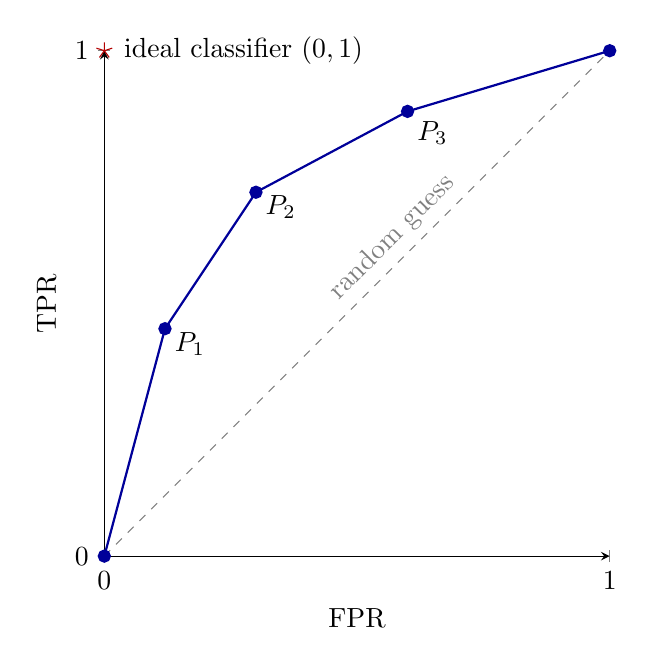
\begin{tikzpicture}
\begin{axis}[
  width=8cm, height=8cm,
  xmin=0, xmax=1, ymin=0, ymax=1,
  xlabel={FPR}, ylabel={TPR},
  xtick={0,1}, ytick={0,1},
  axis lines=left, clip=false]
  \addplot[dashed, gray] coordinates {(0,0) (1,1)};
  \addplot[thick, blue!60!black, mark=*] coordinates {(0,0) (0.12,0.45) (0.3,0.72) (0.6,0.88) (1,1)};
  \node[right] at (axis cs:0.12,0.42) {$P_1$};
  \node[right] at (axis cs:0.3,0.69) {$P_2$};
  \node[below right] at (axis cs:0.6,0.88) {$P_3$};
  \addplot[only marks, mark=star, mark size=3pt, red!70!black] coordinates {(0,1)};
  \node[right] at (axis cs:0.02,1) {ideal classifier $(0,1)$};
  \node[rotate=45, gray, above] at (axis cs:0.6,0.6) {random guess};
\end{axis}
\end{tikzpicture}
\end{center}

To evaluate if the classifier is good we need to evaluate how close we are to the ideal case $(0,1)$. To decide which classifier is closer to the ideal case we can evaluate the \g{area under curve} (AUC): the higher the area, the closer the classifier is to the ideal one. A perfect classifier has $AUC = 1$, while a classifier close to the diagonal (random guessing) has $AUC$ close to $0.5$.
